\section{Stan wiedzy w obszarze przedsięwzięcia}



\subsection{Rekonstrukcja}
Można wyodrębnić gaussian splatting od sfm.

Wirtualne reprezentacje krajobrazów miejskich są coraz bardziej wykorzystywane w różnego rodzaju zadaniach. Mimo rozwoju technik, począwszy od pozyskiwania danych (np. LiDAR), skończywszy na parametrycznych modelach (np. sieci neuronowe), zadanie modelowania pozostawia nierozwiązane problemy wpływające na jakość modelu wynikające z np. trudności akwizycji danych. 
Istnieje wiele sposobów rekonstrukcji które można podzielić ze względu na dane wejściowe, poziom szczegółowości, automatyzację czy też dane wyjściowe. W naszym projekcie rekonstrukcja zachodzi na dwóch etapach - najpierw jako chmura punktów, następnie jako zbiór splatów. 

\subsubsection{SFM}
Opis 'sparse reconstruction'

\subsubsection{Gaussian Splatting}

Popularną techniką rekonstrukcji z chmury punktów jest siatka (ang. mesh), wykorzystana np. w pracy City3D\cite{city3D}. Często jednak uzyskanie dobrej jakości siatki wymaga kombinacji wielu różnych geometrycznych algorytmów. Wraz z rozwojem sztucznej inteligencji zaczęły pojawiać się i w dziedzinie rekonstrukcji rozwiązania wykorzystujące sieci neuronowe - takie jak np. NeRF\cite{nerf}, gdzie informacje o scenie zawarte są w wagach modelu. Niedoskonałością tego rozwiązania jest jednak długi czas trenowania nawet dla sceny jednego obiektu, wahający się od parunastu godzin do paru dni. Z pomocą przychodzą inne metody, jak np. Gaussian Splatting \cite{gaussiansplatting}, który rezygnuje w całości z sieci neuronowej i wykorzystuje zbiór tzw. "splatów" do zbudowania sceny. Jako że w naszym projekcie stawiamy na optymalne wykorzystanie zasobów, to zdecydowaliśmy się na wybór właśnie ostatniej z wymienionych metod. 

\begin{figure}[!htb]
    % images need to be the same size
    \minipage{0.32\textwidth}
      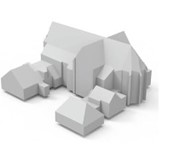
\includegraphics[width=\linewidth]{img/city3dmesh.jpg}
      \caption{City3D - siatka}\label{fig:mesh_example}
    \endminipage\hfill
    \minipage{0.32\textwidth}
      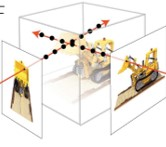
\includegraphics[width=\linewidth]{img/nerfobject.jpg}
      \caption{Nerf - sieć neuronowa}\label{fig:nerf_example}
    \endminipage\hfill
    \minipage{0.32\textwidth}%
      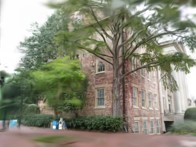
\includegraphics[width=\linewidth]{img/gaussiansplattingobject.jpg}
      \caption{Gaussian Splatting - splat'y}\label{fig:gaussplat_example}
    \endminipage
\end{figure}

Splat (tłum. punkt rozmyty) jest rozszerzeniem punktu i posiada atrybuty
\begin{itemize}
    \item środek (x, y, z)
    \item kolor
    \item przeźroczystość
    \item macierz kowariancji (koduje rotację i skalę)
\end{itemize}

Najlepszy zbiór splatów opisujący scenę jest znajdowany w procesie optymalizacji opisanym poniżej schematem \ref{fig:splatting_algorithm}

\begin{figure}[!htb]
    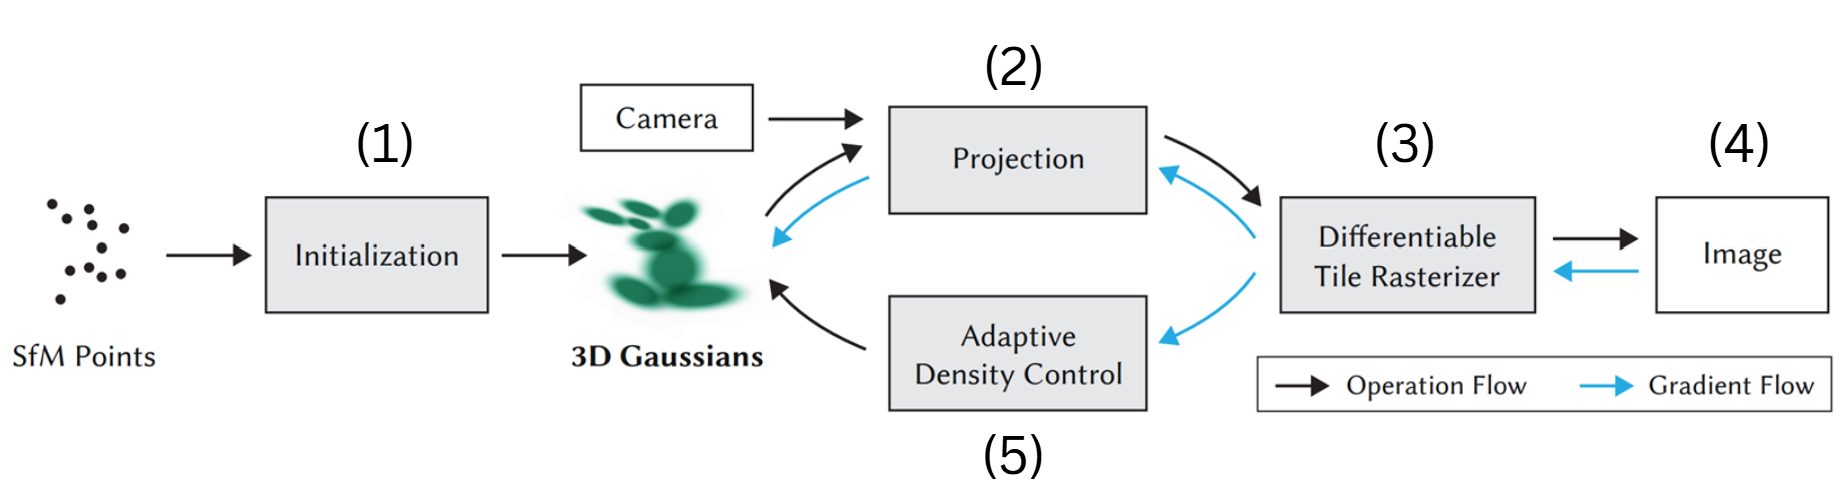
\includegraphics[width=\linewidth]{img/gaussian_splatting_flow.png}
    \caption{Optymalizacja zbioru splatów}\label{fig:splatting_algorithm}
\end{figure}

\begin{enumerate}
    \item Wykorzystanie chmury punktów z rekonstrukcji do inicjalizacji zbioru splatów
    \item Rzutowanie perspektywiczne 3-wymiarowych gaussianów na obraz widziany z danej kamery, czego wynikiem jest zbiór dysków
    \item Renderowanie polegające na akumulowaniu dla każdego piksela wkładu od różnych nachodzących dysków 
    \item Obliczanie funkcji straty - porównanie z prawdziwym obrazkiem z danej kamery
    \item Adaptacja gęstości gaussianów - klonowanie, dzielenie lub usuwanie wg. kryteriów zależnych od strategii
\end{enumerate}

Niestety metoda ta nie pozostaje bez wad. W przypadku dużych zbiorów danych zużycie pamięci może wynieść nawet parę GB, co wymaga dobrej jakości karty graficznej. Inną kwestią jest duża liczba hiperparametrów, które często wymagają ręcznego dostosowania do danej sceny. 

\subsection{Segmentacja}
Warto nadmienić, że nie jest to segmentacja \cite{pointnet}.